~\

\noindent\textbf{Примеры:}
\begin{figure}[h]
	\begin{minipage}[h]{0.49\linewidth}
		\center{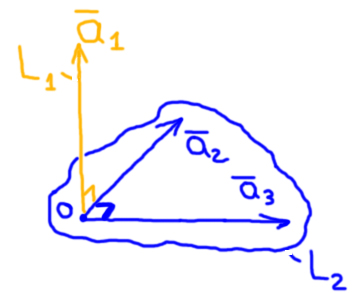
\includegraphics[width=0.666\linewidth]{prim_a_cvet} \\ а)}
	\end{minipage}
	\hfill
	\begin{minipage}[h]{0.49\linewidth}
		\center{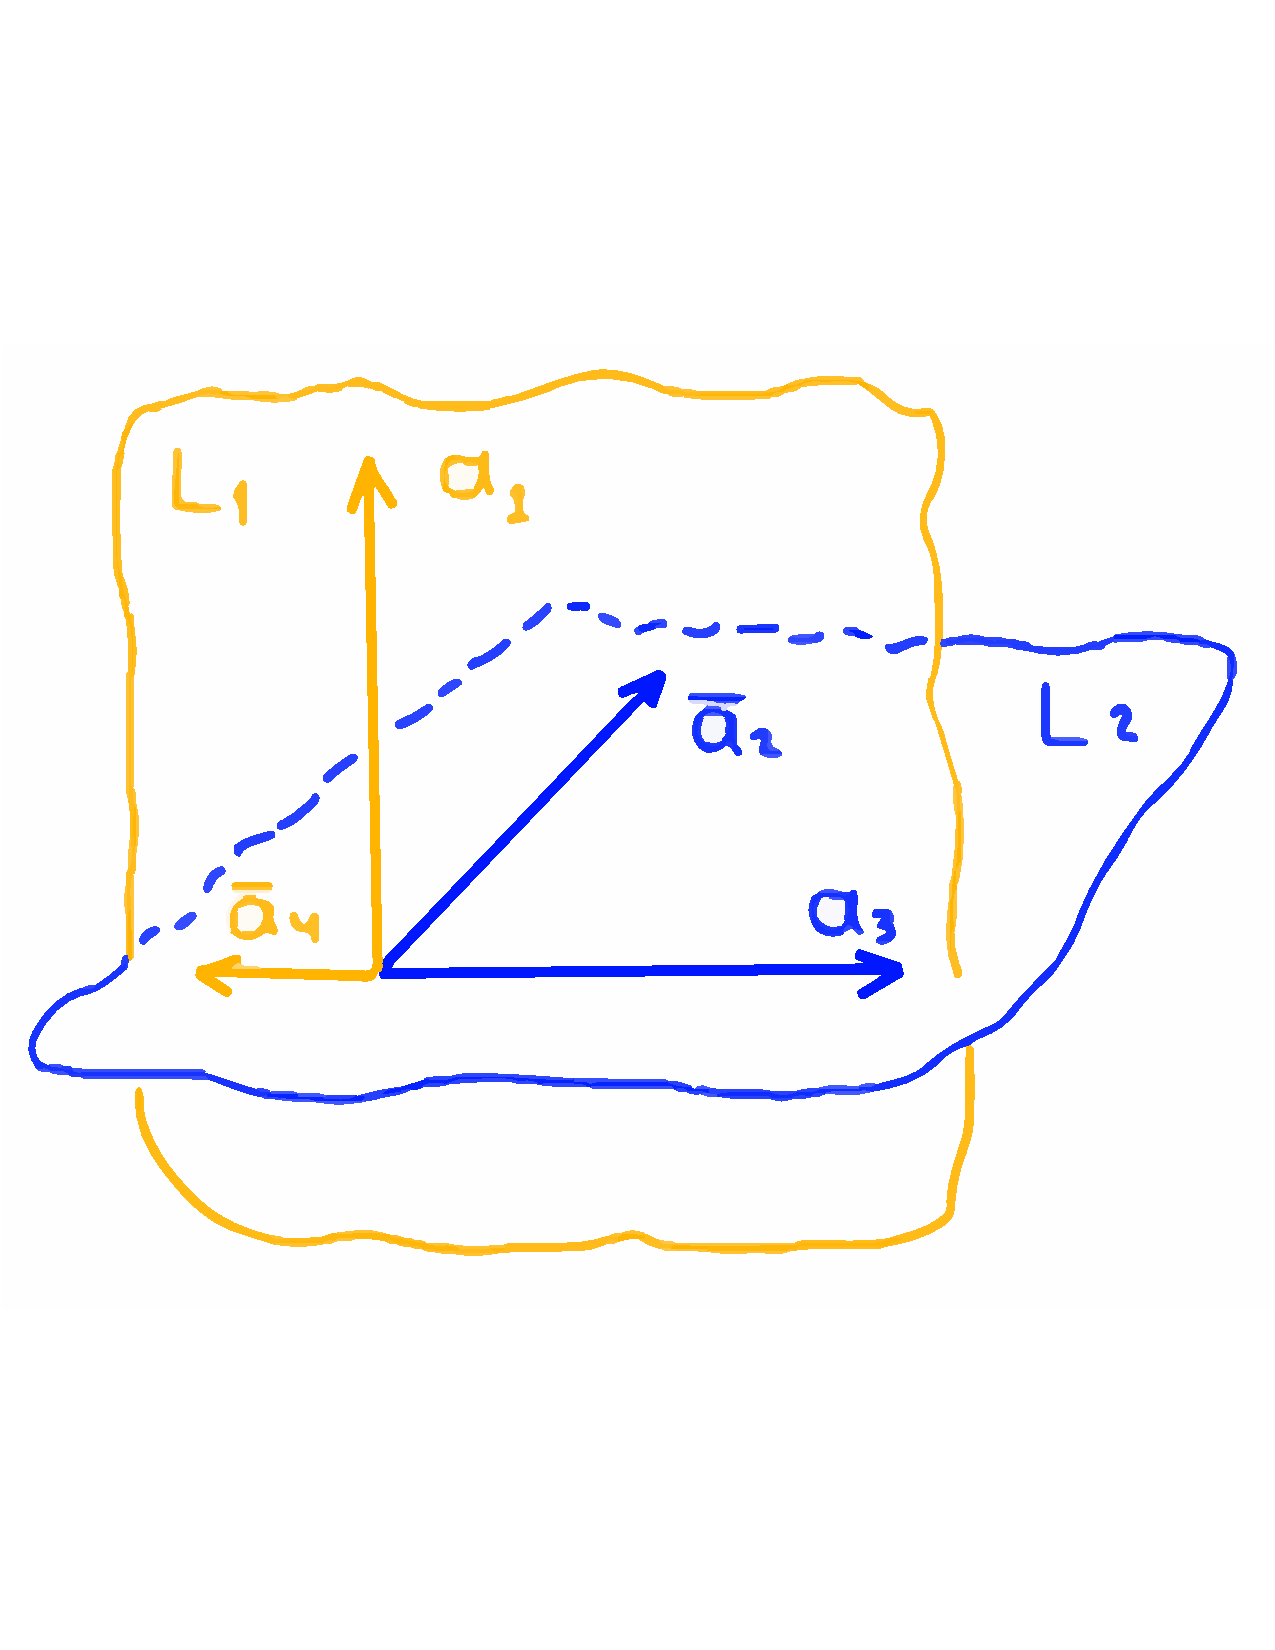
\includegraphics[width=0.8\linewidth]{prim_b_cvet} \\ б)}
	\end{minipage}
	\caption{Рисунки подпространств к примерам а) и б)}
	\label{ris:image1}
\end{figure}

\noindent а) ${\color{orange}L_1}\!:~ <\overline{a}_1\!> \qquad \dim L_1 = 1$\\
\phantom{а)}${\color{blue}L_2}\!:~ <\overline{a}_2, \overline{a}_3\!> \qquad \dim L_2 = 2$\\
В данном случае вектора некомпланарны.\\
$L_1+L_2=<\overline{a}_1, \overline{a}_2, \overline{a}_3\!> = \mathbb{R}^3$\\
$\dim (L_1 +L_2) = 3 = \dim L_1 + \dim L_2$\\
Т.о.
$$
L_1+L_2 = L_1 \oplus L_2
$$
%\begin{wrapfigure}{l}{0.3\linewidth}
%	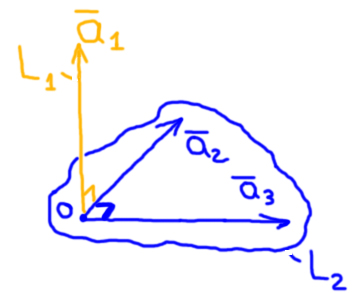
\includegraphics[height=0.2\textheight]{prim_a_cvet}
%	\caption{Рисунок подпространств к примеру а)}
%\end{wrapfigure}
б) ${\color{orange}L_1}\!:~ <\overline{a}_1, \overline{a}_4> \qquad \dim L_1 = 2$\\
${\color{blue}L_2}\!:~ <\overline{a}_2, \overline{a}_3> \qquad \dim L_2 = 2$\\
$L_1+L_2\!:~<\overline{a}_1, \overline{a}_2, \overline{a}_3, \overline{a}_4\!>: \mathbb{R}^3$\\
Но $\dim (L_1+L_2)=3$, т.к. $\overline{a}_4$ можно выкинуть.

В общем случае:
$$
\dim (L_1+L_2) \leq \dim L_1 + \dim L_2
$$
Ответ о размерности даёт \textsf{формула Грассмана}:
$$
\dim (L_1+L_2)=\dim L_1+ \dim L_2 - \dim(L_1\cap L_2).
$$
\section{Понятие проекции вектора на подпространство}
\begin{definition}
	Пусть $\exists a\in L_1,\ b\in L_2, \ x \in L_1+L_2:\ \exists!x = a + b \Leftrightarrow L_1+L_2 = L_1 \oplus L_2$. При этом вектор $a$ называется \textsf{проекцией вектора} $x$ на $L_1$ параллельно $L_2$.  
\end{definition}
\begin{prim}
	Найти проекцию $X(0\ -1\ -1\ 4)^{\text{T}}$ на подпространство $L_1: x_1+x_2+x_3+x_4=0$ вдоль линейной оболочки $L_2\!:~<(1\ -1\ 1\ 0)^{\text{T}}$>.
\end{prim}\\
$L_1: (1\ 1\ 1\ 1\ |\ 0)\Rightarrow
\begin{pmatrix}
x_1\\
x_2\\
x_3\\
x_4\\
\end{pmatrix}
=
\begin{pmatrix*}[r]
-1&-1&-1\\
1&0&0\\
0&1&0\\
0&0&1\\
\end{pmatrix*}
\begin{pmatrix*}[r]
c_1\\
c_2\\
c_3\\
\end{pmatrix*}
$
или
$L_1:
<
\begin{pmatrix*}[r]
-1\\
1\\
0\\
0\\
\end{pmatrix*}
,
\begin{pmatrix*}[r]
-1\\
0\\
1\\
0\\
\end{pmatrix*}
,
\begin{pmatrix*}[r]
-1\\
0\\
0\\
1\\
\end{pmatrix*}
>.
$\\
$
L_2\!:~<\begin{pmatrixr}
1\\-1\\1\\0\\
\end{pmatrixr}>
$\\
Разложим вектор $X$:\\
$$
\begin{pmatrixr}
0\\-1\\-1\\4
\end{pmatrixr}
=\underbrace{
k
\begin{pmatrixr}
1\\-1\\1\\0\\
\end{pmatrixr}
}_{b\in L_2}
+\underbrace{
\alpha
\begin{pmatrixr}
-1\\1\\0\\0\\
\end{pmatrixr}
+\beta
\begin{pmatrixr}
-1\\0\\1\\0\\
\end{pmatrixr}
+\gamma
\begin{pmatrixr}
4\\0\\0\\1\\
\end{pmatrixr}
}_{a\in L_1}
$$
Очевидно, что это уравнение задает нам СЛУ. Составим ее расширенную матрицу и решим систему:\\
$
\left(\begin{array}{rrrr|r}
1&-1&-1&4&0\\
-1&1&0&0&-1\\
1&0&1&0&-1\\
0&0&0&1&4\\
\end{array}\right)
\rightarrow
\begin{pmatrixr}
k\\\alpha\\\beta\\\gamma\\
\end{pmatrixr}
=
\begin{pmatrixr}
2\\1\\-3\\4\\
\end{pmatrixr}.
$\\
Отсюда легко найти, что
$$
x_{\text{пр}}=
\begin{pmatrixr}
0\\-1\\-1\\4\\
\end{pmatrixr}
-2
\begin{pmatrixr}
1\\-1\\1\\0\\
\end{pmatrixr}
=
\begin{pmatrixr}
-2\\1\\-3\\4\\
\end{pmatrixr}.
$$

\begin{prim}
Найти размероность и базис суммы подпространств $U_1$ и $U_2$.
$$
U_1\!:~<
\begin{psm}
1\\0\\-2\\0\\
\end{psm}
,
\begin{psm}
2\\1\\-1\\1
\end{psm}
,
\begin{psm}
3\\2\\0\\2
\end{psm}
>
\quad
U_2:
\left\{
\begin{array}{rrrrl}
x_1&-2x_2&-3x_3&+4x_4&=0\\
3x_1&+x_2&-2x_3&-2x_4&=0\\
\end{array}
\right.
$$
\end{prim}
$
U_1:
\begin{pmatrixr}
1&0&-2&0\\
2&1&-1&1\\
3&2&0&2\\
\end{pmatrixr}
\xrightarrow[(3)-3(1)]{(2)-2(1)}
\begin{pmatrixr}
1&0&-2&0\\
0&1&3&1\\
0&2&6&2\\
\end{pmatrixr}
$\\
Последняя строка ЛЗ со второй, ее можно вычеркнуть $\Rightarrow \dim U_1 = 2$, базис:
$\left\{
\begin{psm}
1\\0\\-2\\0\\
\end{psm}
,
\begin{psm}
0\\1\\3\\1\\
\end{psm}
\right\}.
$\\
Переведём способ задания $U_2$ из СЛУ в линейную оболочку. Для этого решим эту СЛУ:\\
$
\left(\begin{array}{rrrrr}
1&-2&-3&4&0\\
3&1&-2&-2&0\\
\end{array}\right)
\rightarrow
\left(\begin{array}{rrrrr}
1&0&-1&0&0\\
0&1&1&-2&0\\
\end{array}\right)
$\\
$$
\begin{pmatrixr}
x_1\\x_2\\x_3\\x_4\\
\end{pmatrixr}
=
\begin{pmatrixr}
1&0\\
-1&2\\
1&0\\
0&1\\
\end{pmatrixr}
\begin{pmatrixr}
c_1\\c_2\\
\end{pmatrixr}, \quad \dim U_2 = 2, \quad \text{ базис }U_2:\left\{\begin{pmatrixr}
1\\-1\\1\\0\\
\end{pmatrixr}
,
\begin{pmatrixr}
0\\-2\\0\\1\\
\end{pmatrixr}\right\}.
$$
$
U_1+U_2\!:~<
\begin{psm}
1\\0\\-2\\0
\end{psm}
,
\begin{psm}
0\\1\\3\\1\\
\end{psm}
,\begin{psm}
1\\-1\\1\\0\\
\end{psm}
,
\begin{psm}
0\\2\\0\\1\\
\end{psm}
>.
$\\
$
\begin{pmatrixr}
1&0&1&0\\
0&1&-1&2\\
2&3&1&0\\
0&1&0&1\\
\end{pmatrixr}
\xrightarrow{(3)-(1)}
\begin{pmatrixr}
1&0&-&2&0\\
0&1&3&1\\
0&-1&3&0\\
0&2&0&1\\
\end{pmatrixr}
$\\
3 строка ЛЗ с 2 и 4, ее можно вычеркнуть $\Rightarrow \dim(U_1+U_2) = 3$, базис:
$
\left\{
\begin{psm}
1\\0\\-2\\0\\
\end{psm}
,
\begin{psm}
0\\1\\3\\1\\
\end{psm}
,
\begin{psm}
0\\2\\0\\1\\
\end{psm}
\right\}.
$




